
% VLDB template version of 2020-08-03 enhances the ACM template, version 1.7.0:
% https://www.acm.org/publications/proceedings-template
% The ACM Latex guide provides further information about the ACM template

\documentclass[sigconf, nonacm]{acmart}

%% The following content must be adapted for the final version
% leave empty if no availability url should be set
\newcommand\vldbavailabilityurl{https://github.com/emilycourt/reproducibility_project}

\begin{document}
\title{Evaluating Performance of YFilter's Approach to Nested Path Expression Processing}

%%
%% The "author" command and its associated commands are used to define the authors and their affiliations.
\author{Emily Courtney}
\affiliation{%
  \institution{University of Passau}
  \city{Passau}
  \country{Germany}
}
\email{emily.courtney@uni-passau.de}

\maketitle

%%% do not modify the following VLDB block %%
%%% VLDB block start %%%
\ifdefempty{\vldbavailabilityurl}{}{
\vspace{.3cm}
\begingroup\small\noindent\raggedright\textbf{PVLDB Artifact Availability:}\\
The source code, data, and/or other artifacts have been made available at \url{\vldbavailabilityurl}.
\endgroup
}
%%% VLDB block end %%%

\section{Introduction}

YFilter \cite{yfilter} is an XML filtering system that aims to provide fast, on-the-fly matching of XML encoded data to a large number of queries. The development of YFilter builds off insights from the XFilter system~\cite{xfilter}, which was the first published Finite State Machine-based XML filtering approach. YFilter uses a different approach, and combines all of the path queries into a single Nondeterministic Finite Automaton. It exploits similarities of queries by merging common prefixes of the query paths so that they are processed at most once, resulting in significant improvements in structure matching performance.~\cite{yfilter}

The article ``Path Sharing and Predicate Evaluation
for High-Performance XML Filtering''~\cite{yfilter} describes a series of experiments evaluating the performance of YFilter. The experiment being replicated here is an evaluation of the performance of YFilter's approach to processing nested path expressions. In the experiment, YFilter is run repeatedly with different sets of queries. The query sets vary in the number of distinct queries and the number of nested path expression in each query.

While the same source code~\cite{yfilter_source} used in the original study is available, not all of the data artifacts are available, and so we consider this to be a replication as opposed to a reproduction. 

\section{Experiment Setup}

To run the experiment, we require the YFilter program, a set of XML documents, and a set of queries. 

The original study used a set of 200 XML documents, generated using IBM's XML Generator~\cite{IBM_XML}. While the XML documents used in the study are not available, the YFilter project does include a set of XML documents that the original team generated with the same settings. So, in our replication, we choose 200 of these documents.

The set of queries used in the original study is also not availble. However, a query generator is included in the YFilter project, and the workload settings used to generate the query sets are described in detail. So, for our replication, we use the provided query generator and the stated workload settings to produce query sets.

When generating queries, the parameter NP is used to generate a number of nested path expressions in each query~\cite{yfilter}. The experiment evaluates the performance of YFilter as the number of distinct queries is varied from 1000 to 200,000, with NP equal to 1, 2, and 3.

\section{Experiment Results}

The performance metric used is called ``multiquery processing time (MQPT),'' which captures all costs attributable to the filtering algorithms themselves~\cite{yfilter}. MQPT is calculated as the filtering time minus the document parsing time, and this metric is output when the YFilter program runs.

In the original study, a trend was observed from Figure \ref{fig:reference_figure}. As the number of queries grows, MQPT increases to process the first nested path queries. However, processing additional nested paths costs only a little more than processing the first nested paths.~\cite{yfilter}

TODO: include replicated results and comparison. Since the only available data from the original paper is the included table, the comparison will be done by approximating the results from the first table and comparing our results.


\begin{figure}
  \centering
  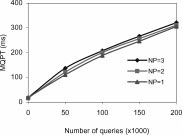
\includegraphics[width=\linewidth]{figures/reference_figure.png}
  \caption{Results from original study~\cite{yfilter}}
  \label{fig:reference_figure}
\end{figure}


%\clearpage

\bibliographystyle{ACM-Reference-Format}
\bibliography{references}

\end{document}
\endinput
